\documentclass[useAMS,usenatbib]{mn2e}
\usepackage{graphicx}
\usepackage{url}
%\usepackage{tikz}
\newcommand{\aap}{Astron. Astrophys.}
\newcommand{\aj}{Astron. J.}
\newcommand{\ao}{Appl. Opt.}
\newcommand{\apj}{Astrophys. J.}
\newcommand{\apjl}{Astrophys. J. Lett.}
\newcommand{\apjs}{Astrophys. J. Suppl.}
\newcommand{\mnras}{Mon. Not. Roy. Ast. Soc.}
\newcommand{\nat}{Nature}
\newcommand{\pasa}{Publ. Ast. Soc. Aust.}
\newcommand{\pasp}{Publ. Ast. Soc. Pac.}
\newcommand{\prl}{Phys. Rev. Lett.}
\newcommand{\msun}{\mathrm{M}_\odot}

\title[2MPZ and LIGO]{Using the 2-MASS Photometric Redshift Survey to optimize LIGO Follow-Up Observations}
\author[Antolini \& Heyl]{Elisa Antolini$^{1}$, Jeremy S. Heyl$^{1}$\thanks{Email:
    heyl@phas.ubc.ca; Canada Research Chair}$^{2}$ \\
  $^{1}$Dipartimento di Fisica e Geologia, Universit\`a degli Studi di Perugia, I-06123 Perugia, Italia \\
  $^{2}$Department of Physics and Astronomy, University of British
  Columbia, 6224 Agricultural Road, Vancouver, BC V6T 1Z1, Canada\\
}
\begin{document}
\date{Accepted ---. Received ---; in original form ---}

\pagerange{\pageref{firstpage}--\pageref{lastpage}} \pubyear{2015}

\maketitle

\label{firstpage}

\begin{abstract}
The initial source localizations from LIGO-Virgo will cover large
areas of sky. Because astrophysical sources of gravitational radiation
are likely to reside in galaxies, it would make sense to search first
in regions where the LIGO-Virgo probability is large and where the
density of galaxies is large as well.  Under the Bayesian prior
assumption that the probability of a gravitational-wave event from a
given region of space is proportional to the density of galaxies
within the probed volume, one can calculate an improved localization
of the position of the source simply by multiplying the LIGO-Virgo
skymap by the density of galaxies in the range of redshifts.  We
propose using the 2-MASS Photometric Redshift Galaxy Catalogue for
this purpose and demonstrate that using it can dramtically reduce the
search region for electromagnetic counterparts.
\end{abstract}

\section{Introduction}

\begin{figure}
  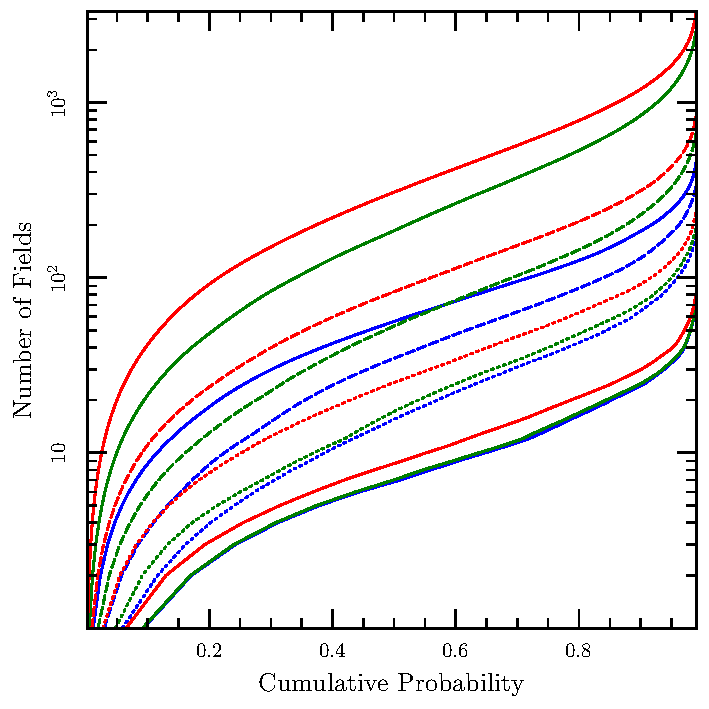
\includegraphics[width=\columnwidth]{T125738_bayestar}
  \caption{The number of fields required to cover the given fraction
    of the probablity region for a simulated LIGO detection (red
    curves without the galaxy map, green curves with a smoothed
    galaxy, blue curves with a raw galaxy map).  The upper solid
    curves use a healpix map with about 200,000 cells, the dashed
    curves have about 50,000 cells, the dotted curves have about
    12,000 cells and lower solid curves have about 3,000 cells,
    corresponding 0.2, 0.8, 3.2 and 13 square-degree fields of view. The redshift range of the galaxy map is $0.03<z<0.04$.}
\end{figure}

This work was supported by the Natural Sciences and Engineering
Research Council of Canada, the Canadian Foundation for Innovation,
the British Columbia Knowledge Development Fund and the Louis and
Bertha Weinstein Research Fund at the University of British Columbia.

\bibliography{obsplan}
\bibliographystyle{apj}


\label{lastpage}
\end{document}
